\documentclass[11pt]{article}
\usepackage[a4paper,  margin=1in]{geometry}
\usepackage{enumitem}
\usepackage{color}
\usepackage{graphicx}
\usepackage{caption}
\usepackage{subcaption}
\usepackage{algorithm}
\usepackage{algorithmicx}
\usepackage{algpseudocode}
\usepackage{listings}
\usepackage{amssymb}
\usepackage{tikz}
\usepackage{pgfplots}

\definecolor{dkgreen}{rgb}{0,0.6,0}
\definecolor{gray}{rgb}{0.5,0.5,0.5}
\definecolor{codebg}{rgb}{0.95,0.95,0.9}
\definecolor{mauve}{rgb}{0.58,0,0.82}

\lstset{frame=tb,
  rulecolor=\color{codebg},
  backgroundcolor=\color{codebg},
  language=C++,
  aboveskip=3mm,
  belowskip=-0.5mm,
  showstringspaces=false,
  columns=flexible,
  basicstyle={\small\ttfamily},
  numbers=none,
  numberstyle=\tiny\color{gray},
  morekeywords={vector},
  keywordstyle=\color{blue},
  commentstyle=\color{dkgreen},
  stringstyle=\color{mauve},
  breaklines=true,
  breakatwhitespace=true,
  tabsize=3
}

\graphicspath{{pic/}}
\setlength\parskip{6pt}
\setlength\parindent{0pt}
\setlength\intextsep{9pt}
\linespread{1}
\renewcommand{\refname}{\vspace{-30pt}}
\renewcommand\floatpagefraction{0.85}

\title{\bf{VFX Project 1\\\large{High Dynamic Range Imaging}}\vspace{-10pt}}
\author{B03901056 Fan-Keng Sun, B03901119 Shang-Wei Chen}
\date{}
  
\begin{document}
\maketitle
\section{Description}
In this project, we assemble high dynamic range (HDR) images from a series of photographs under various exposures, using a popular vision library, OpenCV, for image processing and I/O. The photographs are preprocessed using median threshold bitmap (MTB) algorithm for image alignment. With the aid of tone mapping algorithm, HDR images are reproduced to LDR images in a better human perceptual sense. We learned basic photographing theories and image processing skills from the project. The features we have implemented are:
\vspace{-8pt}
\begin{itemize}
  \itemsep=-2pt
  \item Image alignment: MTB algorithm.
  \item HDR imaging: Paul Debevec's method.
  \item Tone mapping: Erik Reinhard's method.
  \item Exposure fusion: Tom Mertens' method.
  \item Blob removal
  \item Ghost removal: EA Khan's method.
  \item Spotlighting
\end{itemize}
\vspace{-8pt}

\section{Implementation}
\subsection{Environment}
\begin{itemize}
  \itemsep=-2pt
  \item Camera: Sony A6000 (lens: Sony SELP1650)
  \item OS: Linux (Archlinux 4.10, Ubuntu 16.04)
  \item Tools/Libraries: gcc/g++ 6.3.1, OpenCV 3.2 (C++), Boost $>=$ 1.5, Cmake $>=$ 3.0
\end{itemize}

\subsection{Image alignment}
\input{subsection-image-alignment}
\subsection{HDR Imaging}
\input{subsection-hdr-imaging}
\subsection{Tone Mapping}
\input{subsection-tone-mapping}
\subsection{Blob Removal}
Owing to imperfection of original photos or some irregular situations that the above algorithms do not handle, there might be blobs on the photos. We implement blob removal based on a feature in OpenCV libraries, \texttt{cv::SimpleBlobDetector}. Using the following function (need to include \texttt{features2d.hpp})
\begin{lstlisting}
  static Ptr<SimpleBlobDetector> cv::create(
    const SimpleBlobDetector::Params &parameters=SimpleBlobDetector::Params()
  )
\end{lstlisting}
simply convert RGB color to gray scale only, which may not detect the blobs completely; what's more, splitting RGB color into three channels and thresholding by each channel are not effective enough. Hence, we transform RGB color to \textbf{Lab color space} and threshold the image by \textbf{L} (lightness), \textbf{a} (green-red color component), and \textbf{b} (blue-yellow color component) channels separately, which may have better performance for blob detection, and then use the original \texttt{cv::SimpleBlobDetector} functions to detect the blobs.

This feature is realized by the following function in \texttt{src/util.cpp}
\begin{lstlisting}
  void blob_removal(const Mat& pic, Mat& result)
\end{lstlisting}
Since \texttt{cv::SimpleBlobDetector} provides many parameters for blob detection, such as blob size, circularity, inertia ratio, convexity, and for convenience, we create a panel for tuning these parameters (Fig. \ref{fig:blob-panel}). One of the advantages is that we can manually figure out the correctness of blob detection, and thus prevent the detection from some unwanted results if performing automatically. However, iterations is required for completeness since different blobs may have their own threshold values.

\begin{figure}[!ht]
  \centering
  \includegraphics[height=16cm]{blob-panel1}
  \includegraphics[height=16cm]{blob-panel2}
  \caption{Panel for blob removal}
  \label{fig:blob-panel}
\end{figure}

Once the blobs are detected, we approximately fill out these areas with the average colors nearby. For more details, one can refer to \texttt{src/util.hpp} and \texttt{src/util.cpp}. 
\subsection{Ghost Removal}
The feature is realized in the following function
\begin{lstlisting}
  void ghost_removal(const vector<Mat>& pics, int iter, vector<Mat>& result)
\end{lstlisting}
which is an implementation of \textbf{EA Khan's method} \cite{ref:ghost-removal}. The algorithm iteratively calculate the possibility of each pixel based on its weight, and then calculate the weight for the next iteration by its possibility. For a series of $R$ photos under different exposure times, we assign a vector $\textbf{x}_{ijr}=(L, a, b, i, j)\in \mathbb{R}^5$ to each pixel on a photo, where $L$, $a$, $b$ represent its color, $i$, $j$ represent its position, and $r$ represents the number of photo that contains it. Define the neighborhood of the vector $\textbf{x}_{ijr}$
$$F=\{ \textbf{y}_{pqs}|(p,q,s)\in\textbf{N}(\textbf{x}_{ijr}), (p,q)\neq(i,j), s=1,2,\cdots,R \}$$
In the first iteration, define the weight by a hat function (Fig. \ref{fig:hat})
$$w(Z)=1-\left(2\cdot\frac{Z}{255}-1\right)^{12}$$

\begin{figure}[!ht]
\center
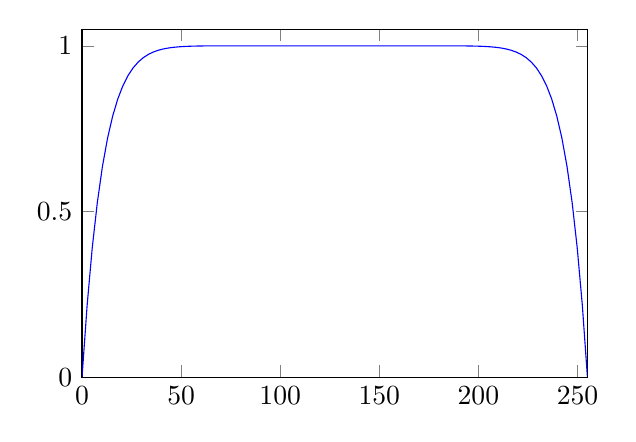
\begin{tikzpicture}
  \begin{axis}[
    domain=0:255,
    xmin=0, xmax=255,
    ymin=0, ymax=1.05,
    samples=100,
    width=8cm, height=6cm
  ]
    \addplot+[mark=none] {1-(2*(x/255)-1)^12};
  \end{axis}
\end{tikzpicture}
\caption{Hat function for ghost removal weighting}
\label{fig:hat}
\end{figure}

where $Z$ is the average value of three channels. Then, calculate the possibility by
$$ 
P(\textbf{x}_{ijr}|F)=
\frac{
  \sum_{p,q,s\in N(\textbf{x}_{ijr})}w_{pqs}K_\textbf{H}(\textbf{x}_{ijr}-\textbf{y}_{pqs})
  }{
    \sum_{p,q,s\in N(\textbf{x}_{ijr})}w_{pqs}
  } 
$$
where
$$K_\textbf{H}(\textbf{x})=|\textbf{H}|^{-1/2}(2\pi)^{-5/2}\exp(-\frac{1}{2}\textbf{x}^T\textbf{H}^{-1}\textbf{x})$$
and $\textbf{H}$ is an identity matrix. Afterwards, calculate the weight for the next iteration
$$w_{pqs, t+1}=w(Z_s(p,q))\cdot P(\textbf{x}_{ijr}|F)$$
in which $w(Z_s(p,q))$ stands for the initial weight.


\subsection{Spotlighting}
Since there might be some objects moving irregularly when shooting photographs, and can barely rebuild the image by the previous ghost removal method, we use the function
\begin{lstlisting}
  void cv::seamlessClone(InputArray src, InputArray dst, InputArray mask, Point p, OutputArray blend, int flags)
\end{lstlisting}
in OpenCV libraries to recover the waving parts in the photos by simply replacing them based on one photo. The feature is realized in the following function
\begin{lstlisting}
  void add_spotlight(vector<Mat>& pics, const vector<double>& para)
\end{lstlisting}
One may refer to \texttt{src/util.cpp} for more detail.

\section{Results}
\subsection{Response Curve}
\begin{figure}[!ht]
\center
\hspace{-45pt}
\subcaptionbox{$\lambda=0.5$}{
  \begin{tikzpicture}
    \begin{axis}[
      domain=0:255,
      xticklabel style={font=\scriptsize},
      yticklabel style={font=\scriptsize},
      xmin=0, xmax=255,
      ymin=-4.5, ymax=3,
      samples=100,
      width=6.5cm, height=5cm
    ]
    \addplot [color=blue, thick] table [x=x, y=y] {data/curveB_5.txt};
    \addplot [color=red, thick] table [x=x, y=y] {data/curveR_5.txt};
    \addplot [color=green, thick] table [x=x, y=y] {data/curveG_5.txt};
    \end{axis}
  \end{tikzpicture}
}
\hspace{-10pt}
\subcaptionbox{$\lambda=5$}{
  \begin{tikzpicture}
    \begin{axis}[
      domain=0:255,
      xticklabel style={font=\scriptsize},
      yticklabel style={font=\scriptsize},
      xmin=0, xmax=255,
      ymin=-4.5, ymax=3,
      samples=100,
      width=6.5cm, height=5cm
    ]
    \addplot [color=blue, thick] table [x=x, y=y] {data/curveB_5.txt};
    \addplot [color=red, thick] table [x=x, y=y] {data/curveR_5.txt};
    \addplot [color=green, thick] table [x=x, y=y] {data/curveG_5.txt};
    \end{axis}
  \end{tikzpicture}
}
\hspace{-10pt}
\subcaptionbox{$\lambda=50$}{
  \begin{tikzpicture}
    \begin{axis}[
      domain=0:255,
      xticklabel style={font=\scriptsize},
      yticklabel style={font=\scriptsize},
      xmin=0, xmax=255,
      ymin=-4.5, ymax=3,
      samples=100,
      width=6.5cm, height=5cm
    ]
    \addplot [color=blue, thick] table [x=x, y=y] {data/curveB_5.txt};
    \addplot [color=red, thick] table [x=x, y=y] {data/curveR_5.txt};
    \addplot [color=green, thick] table [x=x, y=y] {data/curveG_5.txt};
    \end{axis}
  \end{tikzpicture}
}
\hspace{-45pt}
\caption{Response curve for Sony A6000}
\label{fig:response-curve}
\end{figure}



\begin{figure}[!ht]
  \centering
  %\subcaptionbox{Ponzo illusion\vspace{5pt}}{\includegraphics[width=.3\linewidth]{blob-panel}}
  %\caption{782\cite{ref:optical-illusion}}
  \label{distort}
\end{figure}

\section{Reference}
\bibliographystyle{unsrt}
\bibliography{hw1}
\end{document}
